\begin{frame}
	\begin{center}
		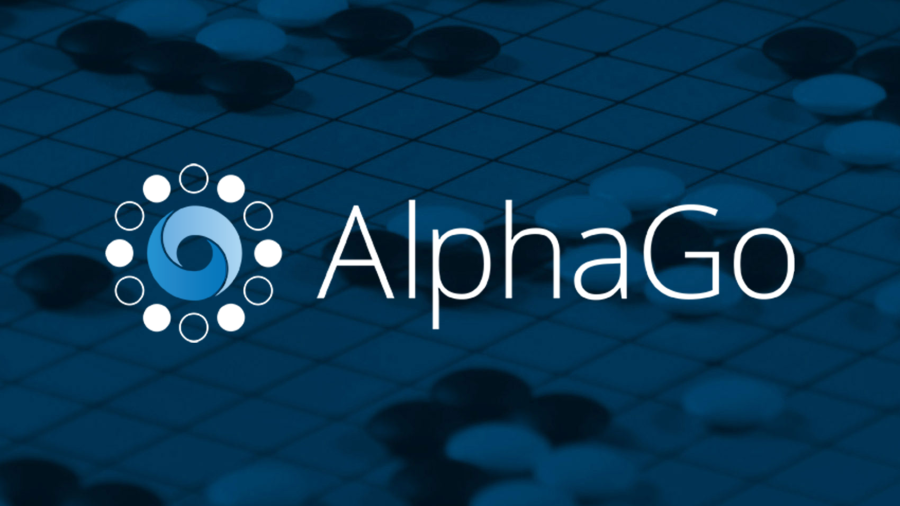
\includegraphics[width=8cm]{ressources/AlphaGoLogo}

	\end{center}
\end{frame}


\begin{frame}{AlphaGo}
	\begin{itemize}
		\item Développé par Google DeepMind
		\item En mars 2016 \textbf{AlphaGo} a battu Lee Sedol, l'un des meilleurs joueurs de Go
		\item Technologies utilisées:
		      \begin{itemize}
			      \item Apprentissage par renforcement
			      \item Réseaux de neurones profonds
			      \item Monte Carlo Tree Search
		      \end{itemize}
	\end{itemize}
\end{frame}


\begin{frame}{AlphaGo}{Structure des technologies utilisés}


\end{frame}
\begin{frame}{AlphaGo}{Apprentissage par renforcement}

	\begin{itemize}
		\item Système de recompense simple : +1 si victoire et -1 si défaite
		\item Entraînement initial supervisé à partir de parties jouées par des humains (30 million de positions différentes)
		\item Deuxième phase d'entraînement non supervisé contre lui-même (\textit{Self-play})
	\end{itemize}

\end{frame}


\begin{frame}{AlphaGo}{Self-play}

	\begin{itemize}
		\item Parties entre la version actuelle de l'agent et une version antérieure aléatoire
		\item
	\end{itemize}

\end{frame}

